\newthought{\textbf{M.IKHSAN - 2020903430016 - TRKJ 3B}}

\newday{\textbf{01 Desember 2022}}
\begin{enumerate}
\item Kendala
% jelaskan kendala dan penyebab yang dialami saat mengikuti praktikum serta solusi atau langkah-langkah yang telah dilakukan
\newline 
1. saat mengintal apache hadoop, apache hadoopnya tidak selesai karena penyimpanan pada ubuntu penuh. jadi, saya menginstal ulang ubuntu untuk menambah penyimpanan
2. masih error saat menjalankan perintah start-dfs.sh 

solusi
\item Kesimpulan
% berikan kesimpulan dari praktikum yang telah dikerjkan

\end{enumerate}

\begin{figure}[!ht]
    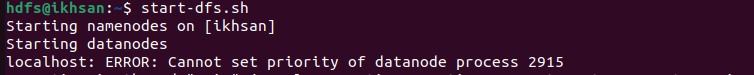
\includegraphics[width=\textwidth]{M.IKHSAN/Capture}
    \caption{error pada perintah start-hdfs.sh}
    \label{gam:Hasil}
\end{figure}

\newday{\textbf{02 Desember 2022}}
\begin{enumerate}
\item Kendala dan Solusi
% jelaskan kendala dan penyebab yang dialami saat mengikuti praktikum serta solusi atau langkah-langkah yang telah dilakukan

\item Kesimpulan
% berikan kesimpulan dari praktikum yang telah dikerjkan

\end{enumerate}

\newday{\textbf{08 Desember 2022}}
\begin{enumerate}
\item Kendala dan Solusi
% jelaskan kendala dan penyebab yang dialami saat mengikuti praktikum serta solusi atau langkah-langkah yang telah dilakukan

\item Kesimpulan
% berikan kesimpulan dari praktikum yang telah dikerjkan

\end{enumerate}


\newday{\textbf{09 Desember 2022}}
\begin{enumerate}
\item Kendala dan Solusi
% jelaskan kendala dan penyebab yang dialami saat mengikuti praktikum serta solusi atau langkah-langkah yang telah dilakukan


\item Kesimpulan
% berikan kesimpulan dari praktikum yang telah dikerjkan
\newline menginstal ulang ubuntu untuk menambah penyimpanan
\end{enumerate}

\newday{\textbf{15 Desember 2022}}
\begin{enumerate}
\item Kendala dan Solusi
% jelaskan kendala dan penyebab yang dialami saat mengikuti praktikum serta solusi atau langkah-langkah yang telah dilakukan

\item Kesimpulan
% berikan kesimpulan dari praktikum yang telah dikerjkan

\end{enumerate}

\newday{\textbf{16 Desember 2022}}
\begin{enumerate}
\item Kendala dan Solusi
% jelaskan kendala dan penyebab yang dialami saat mengikuti praktikum serta solusi atau langkah-langkah yang telah dilakukan

\item Kesimpulan
% berikan kesimpulan dari praktikum yang telah dikerjkan

\end{enumerate}

\newday{\textbf{22 Desember 2022}}
\begin{enumerate}
\item Kendala dan Solusi
% jelaskan kendala dan penyebab yang dialami saat mengikuti praktikum serta solusi atau langkah-langkah yang telah dilakukan

\item Kesimpulan
% berikan kesimpulan dari praktikum yang telah dikerjkan

\end{enumerate}

\newday{\textbf{23 Desember 2022}}
\begin{enumerate}
\item Kendala dan Solusi
% jelaskan kendala dan penyebab yang dialami saat mengikuti praktikum serta solusi atau langkah-langkah yang telah dilakukan

\item Kesimpulan
% berikan kesimpulan dari praktikum yang telah dikerjkan

\end{enumerate}